% ============================================================================
% Lecture 11 (B10): IRBC with DEQNs
% Deep Learning for Solving and Estimating Dynamic Models in Economics and Finance
% Course author: Simon Scheidegger
% ============================================================================

\documentclass[aspectratio=169,11pt]{beamer}

% ---------- Theme and colors ----------
\usecolortheme{dove}
\setbeamertemplate{navigation symbols}{}
\setbeamertemplate{footline}{%
  \hfill\usebeamerfont{page number in head/foot}%
  \usebeamercolor[fg]{normal text}%
  \insertframenumber\,/\,\inserttotalframenumber\kern1em\vskip4pt}
\setbeamerfont{frametitle}{size=\huge}

% ---------- Packages ----------
\usepackage[utf8]{inputenc}
\usepackage[T1]{fontenc}
\usepackage{amsmath,amssymb,amsfonts}
\usepackage{bm}
\usepackage{graphicx}
\usepackage{tikz}
\usetikzlibrary{shapes,arrows.meta,positioning,calc,fit,backgrounds,patterns,decorations.pathreplacing}
\usepackage{pgfplots}
\pgfplotsset{compat=1.18}
\usepackage{booktabs}
\usepackage{hyperref}
\usepackage{multicol}
\usepackage{xcolor}
\usepackage{algorithm}
\usepackage{algorithmic}
\usepackage{listings}

% ---------- Listings style for Python ----------
\lstset{
    language=Python,
    basicstyle=\small\ttfamily,
    keywordstyle=\color{uzhblue}\bfseries,
    commentstyle=\color{uzhgreydark}\itshape,
    stringstyle=\color{darkgreen},
    showstringspaces=false,
    breaklines=true,
    frame=none,
    xleftmargin=0pt,
    aboveskip=4pt,
    belowskip=4pt,
    escapeinside={(*@}{@*)},
}

% ---------- Custom colors ----------
\definecolor{uzhblue}{rgb}{0,0,0.5}
\definecolor{uzhgreylight}{RGB}{236,238,241}
\definecolor{uzhgreydark}{RGB}{81,86,94}
\definecolor{harvardcrimson}{RGB}{153,0,0}
\definecolor{unil@blue}{RGB}{0,140,204}
\definecolor{unil@black}{RGB}{35,31,32}
\definecolor{darkgreen}{RGB}{0,100,0}
\definecolor{darkred}{RGB}{139,0,0}
\definecolor{softblue}{RGB}{70,130,180}
\definecolor{softorange}{RGB}{230,159,0}
\definecolor{softgreen}{RGB}{0,158,115}

% ---------- Set beamer colors ----------
\setbeamercolor{frametitle}{bg=uzhgreylight, fg=uzhblue}
\setbeamercolor{title}{fg=uzhblue}
\setbeamercolor{structure}{fg=uzhblue}
\setbeamercolor{block title}{bg=unil@blue, fg=white}
\setbeamercolor{block body}{bg=uzhgreylight}
\setbeamercolor{block title alerted}{bg=darkred,fg=white}
\setbeamercolor{block body alerted}{bg=red!5}
\setbeamercolor{block title example}{bg=darkgreen,fg=white}
\setbeamercolor{block body example}{bg=green!5}
\setbeamercolor{item}{fg=unil@black}
\setbeamercolor{normal text}{fg=unil@black}

% ---------- Emphasis and hyperlinks ----------
\newcommand{\emphc}[1]{\textcolor{harvardcrimson}{#1}}
\hypersetup{colorlinks,linkcolor=harvardcrimson,urlcolor=harvardcrimson}

% ---------- Math commands ----------
\newcommand{\x}{\bm{x}}
\newcommand{\w}{\bm{w}}
\newcommand{\bb}{\bm{b}}
\newcommand{\z}{\bm{z}}
\newcommand{\W}{\bm{W}}
\newcommand{\X}{\bm{X}}
\renewcommand{\a}{\bm{a}}
\newcommand{\R}{\mathbb{R}}
\newcommand{\E}[1]{\mathbb{E}\!\left[#1\right]}
\DeclareMathOperator*{\argmin}{arg\,min}
\DeclareMathOperator*{\argmax}{arg\,max}

% ---------- Title ----------
\title[Lecture 04 (B03)]{Lecture 04 (B03): IRBC with DEQNs}
\subtitle{Solving nonlinear dynamic stochastic models in 4 to 100+ dimensions}
\author{Simon Scheidegger}
\institute{HEC, University of Lausanne}
\date{}

\begin{document}
% --- Exercise pause badge ---
\newcommand{\exercisepause}{%
  \tikz[baseline=(X.base)]{\node[fill=darkgreen!80!black, text=white,
  rounded corners=2pt, inner sep=3pt, font=\scriptsize\bfseries](X){PAUSE --- 5 min};}}


% ============================================================================
% PART 0: TITLE & OUTLINE
% ============================================================================

% --- Slide 1: Title ---
{\setbeamercolor{background canvas}{bg=uzhgreylight}
\begin{frame}
\titlepage
\vspace{-0.4cm}
\begin{center}
{\footnotesize Based on: Azinovic, Gaegauf \& Scheidegger (2022), \emph{International Economic Review} 63(4), 1471--1525.\\
Brumm, Krause, Schaab \& Scheidegger (2022), ``Sparse Grids for Dynamic Economic Models,'' \emph{Oxford Research Encyclopedia of Economics and Finance}, Oxford University Press.}\\[4pt]
{\footnotesize Materials: \url{https://github.com/sischei/Deep_Learning_for_Solving_And_Estimating_Dynamic_Economic_Models}}
\end{center}
\end{frame}
}

% --- Slide 2: Outline ---
\begin{frame}{Outline}
\begin{enumerate}
    \item \textbf{The IRBC Model}\\
    {\small $N$-country model with irreversible investment, adjustment costs, complete markets.}

    \vspace{0.4em}
    \item \textbf{DEQN Formulation for the IRBC}\\
    {\small State \& policy variables, network architecture, loss function, training algorithm.}

    \vspace{0.4em}
    \item \textbf{Implementation \& Results}\\
    {\small Code walkthrough, convergence, policy functions, economic diagnostics.}
\end{enumerate}
\end{frame}

% --- Slide 3: Roadmap ---
\begin{frame}{Roadmap of This Lecture}
\textbf{Two parts}, with NAS / Loss Normalization (Lecture 12) recommended in between.

\vspace{0.4em}
\begin{columns}[T]
\column{0.48\textwidth}
\textbf{Part A}
\begin{itemize}
    \item \textbf{Part I.} The IRBC model: preferences, production, TFP, adjustment costs, irreversibility, Fischer--Burmeister
    \item Equilibrium system + finger exercise
\end{itemize}

\column{0.48\textwidth}
\textbf{Part B}
\begin{itemize}
    \item \textbf{Part II.} DEQN formulation: states, architecture, loss, Gauss--Hermite, training algorithm
    \item \textbf{Part III.} Implementation: Keras code, convergence, policy functions, validation
    \item Bridge to the production-code DEQN library (Lectures 13--17)
\end{itemize}
\end{columns}
\end{frame}

% ============================================================================
% PART I: THE IRBC MODEL
% ============================================================================

% --- Slide 4: Section Divider ---
\begin{frame}{}
\vfill
\begin{center}
{\Huge \textcolor{uzhblue}{\textbf{Part I}}}\\[12pt]
{\LARGE The IRBC Model}
\end{center}
\vfill
\end{frame}

% --- Slide 5: Why International Models? ---
\begin{frame}{Why International Models?}
\begin{columns}[T]
\column{0.48\textwidth}
\textbf{Key questions in international macro:}
\begin{itemize}
    \item How do \emphc{capital flows} respond to productivity shocks?
    \item What governs \emphc{international risk sharing}?
    \item How do \emphc{trade imbalances} emerge?
\end{itemize}

\vspace{0.5em}
$\Rightarrow$ Need models with $N$ heterogeneous countries.

\vspace{0.3em}
$\Rightarrow$ State space: $2N$ dimensions (capital + TFP per country).

\column{0.48\textwidth}
\begin{center}
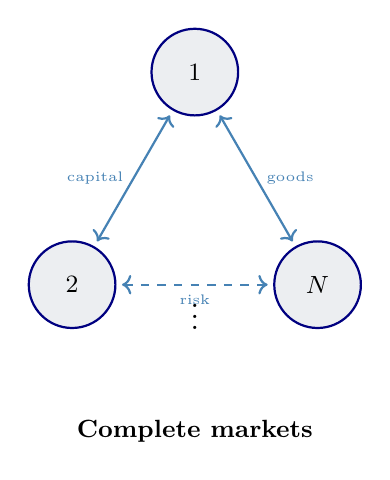
\begin{tikzpicture}[
    country/.style={circle, draw=uzhblue, thick, fill=uzhgreylight,
        minimum size=1.1cm, font=\small},
    flow/.style={<->, thick, softblue, shorten >=2pt, shorten <=2pt}
]
    \node[country] (c1) at (90:1.8) {$1$};
    \node[country] (c2) at (210:1.8) {$2$};
    \node[country] (c3) at (330:1.8) {$N$};
    \node[font=\large] at (270:1.2) {$\vdots$};

    \draw[flow] (c1) -- (c2) node[midway, left, font=\tiny] {capital};
    \draw[flow] (c1) -- (c3) node[midway, right, font=\tiny] {goods};
    \draw[flow, dashed] (c2) -- (c3) node[midway, below, font=\tiny] {risk};

    \node[below=0.3cm, font=\small\bfseries] at (0,-2.2) {Complete markets};
\end{tikzpicture}
\end{center}
\end{columns}
\end{frame}

% --- Slide 5b: IRBC in Macro-Finance ---
\begin{frame}{Why IRBC for Macro-Finance Research?}
\footnotesize
Workhorse for \emphc{open-economy asset pricing} and \emphc{international risk sharing}:

\vspace{0.2em}
\begin{itemize}\itemsep0pt
    \item \textbf{International risk sharing.}  Complete markets imply perfectly correlated consumption; data do not (Backus, Kehoe \& Kydland 1992).
    \item \textbf{Market structure \& welfare.}  Complete vs.\ incomplete markets; welfare cost of missing insurance (Heathcote \& Perri 2002).
    \item \textbf{Capital flows \& current account} from intertemporal savings + heterogeneous productivity.
    \item \textbf{Home bias}: frictionless benchmark for observed portfolio holdings.
    \item \textbf{Macro-financial transmission} via adjustment costs, constraints, Pareto weights.
\end{itemize}
\end{frame}

% --- Slide 5c: IRBC as a computational testbed ---
\begin{frame}{IRBC: Puzzles and Computational Testbed}
\footnotesize
\begin{columns}[T]
\column{0.49\textwidth}
\textbf{Macro-finance puzzles:}
\begin{itemize}\itemsep2pt
    \item \emphc{Consumption-correlation puzzle} (Backus--Kehoe--Kydland 1992):
    complete markets imply $\rho(c^i,c^j)\!\approx\!1$, but in the data $\rho(c^i,c^j)<\rho(y^i,y^j)$.
    \item \emphc{Portfolio home-bias puzzle}: optimal diversification predicts large foreign-equity holdings; observed portfolios are strongly domestic.
    \item \emphc{Real-exchange-rate (RER) volatility} (Backus--Smith): the ratio of price levels $P^j/P^i$ is far more volatile than the consumption ratio $c^j/c^i$; IRBC with nontraded goods (Stockman \& Tesar, 1995) reproduces this.
\end{itemize}

\column{0.49\textwidth}
\textbf{Computational testbed:}
\begin{itemize}\itemsep0pt
    \item State dim.\ \emphc{linear} in $N$: $2N$.
    \item Smooth but \emphc{highly nonlinear}.
    \item \emphc{Planner} gives a clean target.
    \item Benchmark for projection methods (Krueger \& Kubler 2004; Brumm \& Scheidegger 2017).
\end{itemize}
\end{columns}
\end{frame}

% --- Slide 6: Model Overview ---
\begin{frame}{Model Overview}
\textbf{International Real Business Cycle (IRBC) model} --- Backus, Kehoe \& Kydland (1992); here with the DEQN-style extensions of Azinovic, Gaegauf \& Scheidegger (2022):

\vspace{0.5em}
\begin{itemize}
    \item $N$ countries, each with \emphc{country-specific capital} $k^j$ and \emphc{TFP} $z^j$
    \item \emphc{Complete markets}: a social planner allocates resources with Pareto weights $\tau^j$
    \item \emphc{Irreversible investment}: $I^j \geq 0$ (cannot disinvest)
    \item \emphc{Capital adjustment costs}: $\Gamma^j = \frac{\kappa}{2} k^j \!\left(\frac{k^{j\prime}}{k^j} - 1\right)^{\!2}$
\end{itemize}

\vspace{0.5em}
\begin{block}{Dimensionality}
State: $\bm{s} = (k^1, \ldots, k^N, z^1, \ldots, z^N) \in \R^{2N}$\\
Policy: $(k^{1\prime}, \ldots, k^{N\prime}, \lambda, \mu^1, \ldots, \mu^N) \in \R^{2N+1}$
\end{block}
\end{frame}

% --- Slide 7: Preferences ---
\begin{frame}{Preferences}
Each country $j$ has \emphc{CRRA utility}:
\[
u^j(c) = \frac{c^{\,1 - 1/\gamma_j}}{1 - 1/\gamma_j}
\]

\vspace{0.3em}
\begin{itemize}
    \item $\gamma_j$: intertemporal elasticity of substitution for country $j$
    \item \emphc{Heterogeneous} across countries: $\gamma_j$ linearly spaced in $[\gamma_{\min}, \gamma_{\max}]$
    \item $\gamma_{\min} = 0.25$, $\gamma_{\max} = 1.0$ (risk aversion $= 1/\gamma_j$ ranges from 1 to 4)
\end{itemize}

\vspace{0.5em}
\textbf{Social planner} maximizes with Pareto weights $\tau^j$:
\[
\max \; \sum_{t=0}^{\infty} \beta^t \, \E{\sum_{j=1}^{N} \tau^j \, u^j(c_t^j)}
\]
\end{frame}

% --- Slide 8: Production ---
\begin{frame}{Production}
Each country $j$ produces a single good:
\[
Y^j = A_{\text{tfp}} \cdot \exp(z^j) \cdot (k^j)^\zeta
\]

\vspace{0.3em}
\textbf{Calibration of $A_{\text{tfp}}$:} chosen so that the \emphc{steady state} is consistent with $k_{ss} = 1$:
\[
\boxed{A_{\text{tfp}} = \frac{1 - \beta(1-\delta)}{\zeta \cdot \beta}}
\]

\vspace{0.5em}
\begin{center}
\begin{tabular}{ll}
\toprule
\textbf{Parameter} & \textbf{Value} \\
\midrule
$\zeta$ (capital share) & 0.36 \\
$\beta$ (discount factor) & 0.99 \\
$\delta$ (depreciation) & 0.01 \\
\bottomrule
\end{tabular}
\end{center}
\end{frame}

% --- Slide 9: TFP Process ---
\begin{frame}{TFP Process}
\begin{columns}[T]
\column{0.48\textwidth}
Log TFP follows an \emphc{AR(1)} with common and idiosyncratic shocks:
\[
z^{j\prime} = \rho_z \, z^j + \sigma_e \bigl(\varepsilon^j + \varepsilon^{\text{agg}}\bigr)
\]

\vspace{0.3em}
\begin{itemize}
    \item $\varepsilon^j \sim \mathcal{N}(0,1)$: country-specific
    \item $\varepsilon^{\text{agg}} \sim \mathcal{N}(0,1)$: aggregate shock
    \item Total: $N+1$ independent shocks
\end{itemize}

\vspace{0.3em}
{\small $\rho_z = 0.95$, $\sigma_e = 0.01$}

\column{0.48\textwidth}
\begin{center}
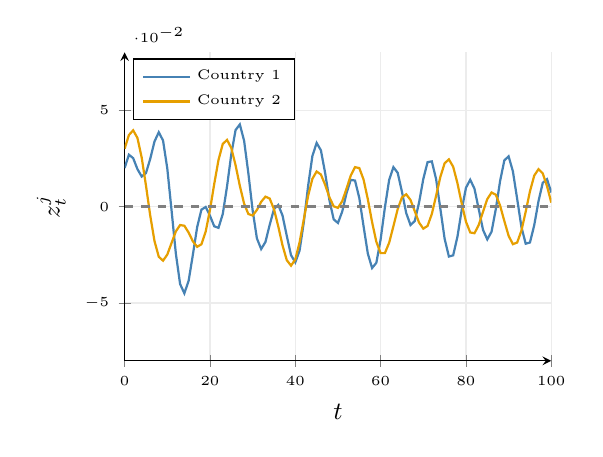
\begin{tikzpicture}
\begin{axis}[
    width=7cm, height=5.5cm,
    xlabel={$t$}, ylabel={$z^j_t$},
    xlabel style={font=\small},
    ylabel style={font=\small},
    tick label style={font=\tiny},
    xmin=0, xmax=100, ymin=-0.08, ymax=0.08,
    grid=major, grid style={gray!15},
    legend style={font=\tiny, at={(0.02,0.98)}, anchor=north west},
    axis lines=left,
]
    \addplot[thick, softblue, domain=0:100, samples=101]
        {0.04*sin(deg(x*0.3))*exp(-0.02*x) + 0.02*cos(deg(x*0.7))};
    \addlegendentry{Country 1}
    \addplot[thick, softorange, domain=0:100, samples=101]
        {0.03*cos(deg(x*0.25))*exp(-0.015*x) + 0.015*sin(deg(x*0.6))};
    \addlegendentry{Country 2}
    \addplot[thick, dashed, gray, domain=0:100]{0};
\end{axis}
\end{tikzpicture}\\
{\tiny Stylized TFP sample paths}
\end{center}
\end{columns}
\end{frame}

% --- Slide 10: Adjustment Costs ---
\begin{frame}{Capital Adjustment Costs}
\begin{columns}[T]
\column{0.48\textwidth}
Changing the capital stock is \emphc{costly} ($\kappa = 0.5$):
\[
\Gamma^j = \frac{\kappa}{2}\, k^j \!\left(\frac{k^{j\prime}}{k^j} - 1\right)^{\!2}
\]

\textbf{Key derivatives:}
\begin{align*}
\frac{\partial \Gamma}{\partial k'} &= \kappa \left(\frac{k'}{k} - 1\right) \\[2pt]
\frac{\partial \Gamma}{\partial k} &= -\frac{\kappa}{2}\left(\frac{k'}{k} - 1\right)\!\left(\frac{k'}{k} + 1\right)
\end{align*}

{\footnotesize\textbf{Role:} smooth investment, break Tobin's $q\!=\!1$, and dampen cross-country \emphc{capital flows}.}

\column{0.48\textwidth}
\begin{center}
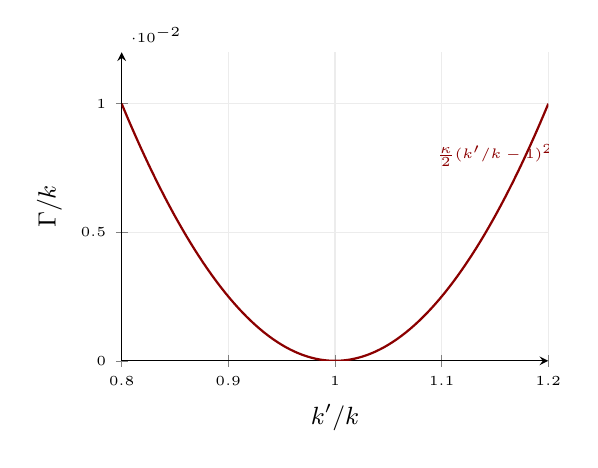
\begin{tikzpicture}
\begin{axis}[
    width=7cm, height=5.5cm,
    xlabel={$k'/k$}, ylabel={$\Gamma / k$},
    xlabel style={font=\small},
    ylabel style={font=\small},
    tick label style={font=\tiny},
    xmin=0.8, xmax=1.2, ymin=0, ymax=0.012,
    grid=major, grid style={gray!15},
    axis lines=left,
]
    \addplot[thick, darkred, domain=0.8:1.2, samples=100]
        {0.25*(x-1)^2};
    \node[font=\tiny, darkred] at (axis cs:1.15,0.008) {$\frac{\kappa}{2}(k'/k-1)^2$};
\end{axis}
\end{tikzpicture}\\
{\tiny Adjustment cost per unit of capital}
\end{center}
\end{columns}
\end{frame}

% --- Slide 11: Putting It Together ---
\begin{frame}{Putting It Together: The Complete Model}
\footnotesize
\textbf{Primitives} (from the previous slides):
\begin{align*}
\text{Preferences:}   &\quad U^j(c) = \tfrac{c^{\,1 - 1/\gamma_j}}{1 - 1/\gamma_j} \\[1pt]
\text{Production:}    &\quad Y_t^j = A_{\mathrm{tfp}}\,\exp(z_t^j)\,(k_t^j)^{\zeta} \\[1pt]
\text{TFP process:}   &\quad z_{t+1}^j = \rho_z\, z_t^j + \sigma_e\bigl(\varepsilon_{t+1}^j + \varepsilon_{t+1}^{\mathrm{agg}}\bigr) \\[1pt]
\text{Adjustment cost:}&\quad \Gamma_t^j = \tfrac{\kappa}{2}\, k_t^j \bigl(k_{t+1}^j/k_t^j - 1\bigr)^{2}
\end{align*}

\textbf{Constraints:}
\begin{align*}
\text{Aggregate resource (ARC):} &\quad \sum_{j=1}^{N}\!\Bigl[ Y_t^j + (1-\delta)\, k_t^j - k_{t+1}^j - \Gamma_t^j - c_t^j \Bigr] = 0 \\[2pt]
\text{Irreversibility:} &\quad I_t^j \equiv k_{t+1}^j - (1-\delta)\, k_t^j \;\geq\; 0 \qquad \forall\, j = 1,\ldots,N
\end{align*}

\smallskip
The planner chooses $\{c_t^j, k_{t+1}^j\}_{j,t}$ subject to these constraints.
\end{frame}

% --- Slide 12: Planner's Problem (dynamic optimization) ---
\begin{frame}{Planner's Problem (Dynamic Optimization)}
\footnotesize
\[
\max_{\{c_t^j,\, k_{t+1}^j\}} \;\; \E{\sum_{t=0}^{\infty} \beta^{t} \sum_{j=1}^{N} \tau^j \, \frac{(c_t^j)^{1 - 1/\gamma_j}}{1 - 1/\gamma_j}}
\]
\textbf{subject to:}
\begin{align*}
\text{ARC:} &\quad \sum_{j=1}^{N} \Bigl[ Y_t^j + (1-\delta)\,k_t^j - k_{t+1}^j - \Gamma_t^j - c_t^j \Bigr] = 0 \\[2pt]
\text{Irreversibility:} &\quad k_{t+1}^j - (1-\delta)\,k_t^j \;\geq\; 0 \qquad \forall\, j \\[2pt]
\text{Production:} &\quad Y_t^j = A_{\mathrm{tfp}}\exp(z_t^j)\,(k_t^j)^{\zeta} \\[2pt]
\text{TFP:}         &\quad z_{t+1}^j = \rho_z\, z_t^j + \sigma_e\bigl(\varepsilon_{t+1}^j + \varepsilon_{t+1}^{\mathrm{agg}}\bigr)
\end{align*}

\smallskip
Pareto weights $\tau^j$ allocate welfare across countries. We now \emph{attach multipliers} to the constraints to obtain the first-order conditions.
\end{frame}

% --- Slide 13: Lagrangian and multipliers ---
\begin{frame}{The Lagrangian: Attaching Multipliers}
\footnotesize
Attach one multiplier per active constraint of the planner's problem:
\begin{itemize}\itemsep2pt
    \item $\lambda_t$ on the aggregate resource constraint --- the \emphc{shadow price of world output} at date $t$.
    \item $\mu_t^j \geq 0$ on country $j$'s irreversibility --- the \emphc{shadow price of being unable to disinvest}.
\end{itemize}

\[
\mathcal{L} \;=\; \E{\,\sum_{t=0}^{\infty} \beta^{t}\!\left[\,
  \sum_{j} \tau^j \tfrac{(c_t^j)^{1-1/\gamma_j}}{1-1/\gamma_j}
  + \lambda_t\!\sum_{j}\!\bigl(Y_t^j + (1-\delta) k_t^j - k_{t+1}^j - \Gamma_t^j - c_t^j\bigr)
  + \sum_{j}\! \mu_t^j \bigl(k_{t+1}^j - (1-\delta) k_t^j\bigr)
\right]\,}
\]

\smallskip
\textbf{Economic reading:}
\begin{itemize}\itemsep1pt
    \item $\lambda_t$ high $\Rightarrow$ world resources scarce $\Rightarrow$ every country cuts consumption.
    \item $\mu_t^j > 0$ only when country $j$'s irreversibility constraint \emph{binds}.
\end{itemize}
\end{frame}

% --- Slide 14: KKT conditions for irreversibility ---
\begin{frame}{KKT Conditions for Irreversibility}
With the multipliers $\mu_t^j$ now defined, optimality of the planner's choice of $k_{t+1}^j$ together with $\mu_t^j \geq 0$ yields the \emphc{complementary slackness} structure:
\[
\mu^j \;\geq\; 0, \qquad I^j \;\geq\; 0, \qquad \mu^j \cdot I^j \;=\; 0.
\]

\smallskip
\textbf{Economic reading:}
\begin{itemize}\itemsep2pt
    \item $I^j > 0$ (agent invests): constraint slack $\Rightarrow \mu^j = 0$.
    \item $I^j = 0$ (constraint binds): $\mu^j \geq 0$ records the shadow value of enforcing $I^j \geq 0$.
\end{itemize}

\vspace{0.3em}
\textbf{Numerical problem:} KKT involves $\min/\max$ --- \emphc{non-differentiable}, incompatible with SGD. Next slide: smooth it via the Fischer--Burmeister function.
\end{frame}

% --- Slide 12: Fischer-Burmeister ---
\begin{frame}{Fischer--Burmeister Complementarity Function}
\begin{columns}[T]
\column{0.48\textwidth}
\textbf{Problem:} KKT conditions involve \emphc{non-smooth} min/max operators.

\vspace{0.3em}
\textbf{Solution:} use a smoothed \emphc{Fischer--Burmeister} (FB) residual:
\[
\text{FB}_\varepsilon(\mu, I) = \mu + I - \sqrt{\mu^2 + I^2 + \varepsilon^2}
\]

\vspace{0.2em}
{\small $\varepsilon > 0$ small for numerical stability.}

\vspace{0.3em}
$\text{FB}_0(\mu, I) = 0$ $\Leftrightarrow$ $\mu \geq 0$, $I \geq 0$, $\mu \cdot I = 0$.  For $\varepsilon>0$, this exact zero set is slightly smoothed near the origin.

\vspace{0.2em}
$\Rightarrow$ For $\varepsilon>0$, \emphc{differentiable} everywhere---compatible with SGD.

\column{0.48\textwidth}
\begin{center}
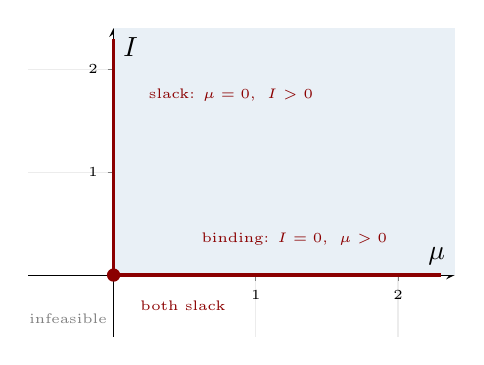
\begin{tikzpicture}
\begin{axis}[
    width=7cm, height=5.5cm,
    xlabel={$\mu$}, ylabel={$I$},
    xlabel style={font=\small, at={(axis description cs:1.02,0.5)}, anchor=west},
    ylabel style={font=\small, at={(axis description cs:0.5,1.04)}, anchor=south, rotate=-90},
    tick label style={font=\tiny},
    xmin=-0.6, xmax=2.4, ymin=-0.6, ymax=2.4,
    grid=major, grid style={gray!15},
    axis lines=middle,
]
    % Feasible quadrant shading
    \fill[softblue!12] (axis cs:0,0) rectangle (axis cs:2.4,2.4);
    % Zero set of FB: the two positive axes (L-shape)
    \addplot[very thick, darkred, domain=0:2.3, samples=2] ({x},{0});
    \addplot[very thick, darkred, domain=0:2.3, samples=2] ({0},{x});
    % Origin marker
    \fill[darkred] (axis cs:0,0) circle (2.4pt);
    % Annotations on each arm (placed in feasible interior so they don't hit the axes)
    \node[font=\tiny, darkred, anchor=south west] at (axis cs:0.55,0.20)
        {binding: $I = 0$,\; $\mu > 0$};
    \node[font=\tiny, darkred, anchor=south west] at (axis cs:0.18,1.6)
        {slack: $\mu = 0$,\; $I > 0$};
    \node[font=\tiny, darkred, anchor=west] at (axis cs:0.12,-0.30) {both slack};
    \node[font=\tiny, gray] at (axis cs:-0.32,-0.42) {infeasible};
\end{axis}
\end{tikzpicture}\\[2pt]
{\scriptsize Red ``L'' $=$ zero set of $\mathrm{FB}$. Every point on it satisfies KKT: one of $\mu, I$ is zero, the other is $\geq 0$. Off the L, $\mathrm{FB} \neq 0$ and the loss penalizes the deviation.}
\end{center}
\end{columns}
\end{frame}

% --- Slide 16: FOC: Consumption Sharing ---
\begin{frame}{FOC: Consumption Sharing}
\textbf{First-order condition} w.r.t.\ $c^j$:
\[
\tau^j \cdot (c^j)^{-1/\gamma_j} = \lambda
\]
where $\lambda$ is the \emphc{shadow price} of the aggregate resource constraint.

\vspace{0.5em}
\textbf{Solving for consumption:}
\[
\boxed{c^j = \left(\frac{\lambda}{\tau^j}\right)^{-\gamma_j}}
\]

\vspace{0.5em}
\begin{itemize}
    \item $\lambda$ is the \emphc{single} policy variable governing consumption allocation
    \item Higher $\lambda$ $\Rightarrow$ resources are scarcer $\Rightarrow$ lower consumption
    \item Countries with higher $\gamma_j$ (lower risk aversion) respond more to $\lambda$
\end{itemize}
\end{frame}

% --- Slide 15: FOC: Euler Equation ---
\begin{frame}{FOC: Euler Equation}
\textbf{First-order condition} w.r.t.\ $k^{j\prime}$:
\[
\lambda\,(1 + \Gamma_{k'}) = \beta\,\E{\lambda' \cdot \text{MPK}^{j\prime} - (1-\delta)\,\mu^{j\prime}} + \mu^j
\]

where:
\begin{itemize}
    \item $\Gamma_{k'} = \kappa\!\left(\frac{k'}{k} - 1\right)$ is the marginal adjustment cost
    \item $\text{MPK}^j = 1 - \delta + \zeta A_{\text{tfp}} \exp(z^j)\,(k^j)^{\zeta-1} - \frac{\partial \Gamma}{\partial k}$
    \item $\mu^j$ is the \emphc{irreversibility multiplier}
    \item The term $(1-\delta)\,\mu^{j\prime}$ captures the \emphc{shadow value} if the constraint binds tomorrow
\end{itemize}
\end{frame}

% --- Slide 16: Euler in Relative Error ---
\begin{frame}{Euler Equation: Relative Error Form}
Rearranging the Euler equation into \emphc{relative error} form:

\[
\boxed{
\frac{\beta\,\E{\lambda' \cdot \text{MPK}^{j\prime} - (1-\delta)\,\mu^{j\prime}} + \mu^j}{\lambda\,(1 + \Gamma_{k'})} - 1 = 0
}
\]

\vspace{0.5em}
\textbf{Why relative error?}
\begin{itemize}
    \item All $N$ Euler equations are \emphc{scale-free}
    \item Residuals can be interpreted as \emphc{percentage errors} in the optimality condition
    \item A residual of $10^{-3}$ means the agent is off by 0.1\%
\end{itemize}
\end{frame}

% --- Slide 17: Aggregate Resource Constraint ---
\begin{frame}{Aggregate Resource Constraint}
All output must be allocated to consumption, investment, and adjustment costs:

\[
\boxed{
\sum_{j=1}^{N} \Bigl[\underbrace{Y^j + (1-\delta)\,k^j}_{\text{resources}} - \underbrace{k^{j\prime}}_{\text{investment}} - \underbrace{\Gamma^j}_{\text{adj.\ cost}} - \underbrace{c^j}_{\text{consumption}}\Bigr] = 0
}
\]

\vspace{0.5em}
\begin{itemize}
    \item This is a \emphc{single} equation (not $N$ separate ones)
    \item Under complete markets, goods flow freely between countries
    \item Consumption $c^j$ is determined by $\lambda$ and the Pareto weights
\end{itemize}
\end{frame}

% --- Slide 18: Complementarity Conditions ---
\begin{frame}{Complementarity Conditions}
For each country $j$, the Fischer--Burmeister condition enforces irreversibility:

\[
\text{FB}_{\varepsilon}(\mu^j, I^j)
= \mu^j + I^j - \sqrt{(\mu^j)^2 + (I^j)^2 + \varepsilon^2} = 0
\]

where $I^j = k^{j\prime} - (1-\delta)\,k^j$.

\vspace{0.5em}
\textbf{Total system:}
\begin{center}
\begin{tabular}{lcc}
\toprule
\textbf{Equation} & \textbf{Count} & \textbf{Unknown} \\
\midrule
Euler equations & $N$ & $k^{1\prime}, \ldots, k^{N\prime}$ \\
Aggregate resource constraint & $1$ & $\lambda$ \\
Fischer--Burmeister & $N$ & $\mu^1, \ldots, \mu^N$ \\
\midrule
\textbf{Total} & $\bm{2N+1}$ & $\bm{2N+1}$ \\
\bottomrule
\end{tabular}
\end{center}
\end{frame}

% --- Slide 19: Summary: Equilibrium System ---
\begin{frame}{Summary: Equilibrium System}
\textbf{Well-posed system:} $2N+1$ equations in $2N+1$ unknowns.

\vspace{0.5em}
\begin{center}
\begin{tabular}{rrrr}
\toprule
$N$ & \textbf{States} & \textbf{Policies} & \textbf{Equations} \\
\midrule
2 & 4 & 5 & 5 \\
4 & 8 & 9 & 9 \\
10 & 20 & 21 & 21 \\
50 & 100 & 101 & 101 \\
100 & 200 & 201 & 201 \\
\bottomrule
\end{tabular}
\end{center}

\vspace{0.3em}
\begin{itemize}
    \item Dimensions grow \emphc{linearly} in $N$---no combinatorial explosion
    \item Traditional grid methods: $\mathcal{O}(n^{2N})$ grid points
    \item DEQNs: a single neural network, trained via SGD
\end{itemize}
\end{frame}

% --- Finger Exercise: IRBC ---
\begin{frame}{\exercisepause{} Finger Exercise: IRBC Euler Equations}
\begin{exampleblock}{Exercise}
Consider the 2-country IRBC model. Suppose we \emphc{double} the capital depreciation rate $\delta$ from the baseline $0.01$ to $0.02$.
\begin{enumerate}
    \item Without running any code: will the steady-state capital stock in each country \emph{increase} or \emph{decrease}? Why?
    \item Will the optimal savings rate (investment / output) increase or decrease?
    \item Open notebook \texttt{01\_IRBC\_DEQN.ipynb}, change $\delta$, and verify your prediction.
\end{enumerate}
\end{exampleblock}
\end{frame}

\begin{frame}{Solution: IRBC Euler Equations}
\begin{block}{Answer}
\begin{enumerate}
    \item Steady-state capital \emphc{decreases}. In steady state, the Euler equation implies $r = 1/\beta - 1 + \delta$. Higher $\delta$ means higher required return $r$, which (with diminishing returns) requires lower $k^*$.
    \item The savings rate \emphc{increases}. More capital depreciates each period, so a larger fraction of output must be reinvested just to maintain the (lower) capital stock.
    \item In the notebook: changing $\delta$ from $0.01$ to $0.02$ should show the policy function shifting down (lower capital) and the investment share rising.
\end{enumerate}
\end{block}
\end{frame}

% ============================================================================
% PART II: DEQN FORMULATION
% ============================================================================

% --- Slide 20: Section Divider ---
\begin{frame}{}
\vfill
\begin{center}
{\Huge \textcolor{uzhblue}{\textbf{Part II}}}\\[12pt]
{\LARGE DEQN Formulation for the IRBC}
\end{center}
\vfill
\end{frame}

% --- Slide 21: State & Policy Variables ---
\begin{frame}{State \& Policy Variables}
\begin{center}
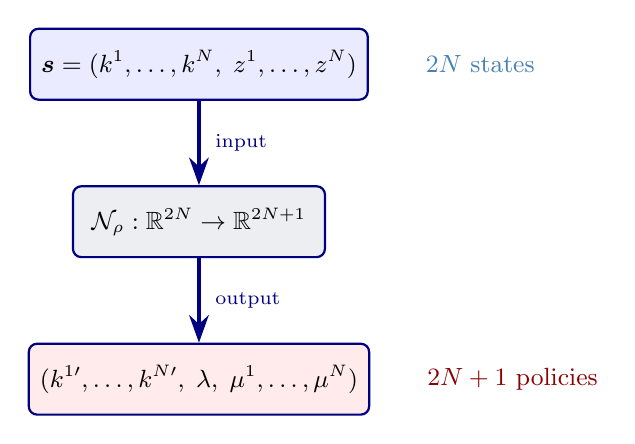
\begin{tikzpicture}[
    mlstep/.style={rectangle, draw=uzhblue, thick, fill=uzhgreylight,
        minimum width=3.2cm, minimum height=0.9cm, font=\small,
        rounded corners=3pt, inner sep=4pt},
    arr/.style={-{Stealth[length=3.5mm, width=2.5mm]}, very thick, uzhblue}
]
    \node[mlstep, fill=blue!8] (state) at (0, 0)
        {$\bm{s} = (k^1, \ldots, k^N,\; z^1, \ldots, z^N)$};
    \node[mlstep] (nn) at (0, -2.0)
        {$\mathcal{N}_\rho : \R^{2N} \to \R^{2N+1}$};
    \node[mlstep, fill=red!8] (policy) at (0, -4.0)
        {$(k^{1\prime}, \ldots, k^{N\prime},\; \lambda,\; \mu^1, \ldots, \mu^N)$};

    \draw[arr] (state) -- node[right, font=\scriptsize, uzhblue, xshift=2pt] {input} (nn);
    \draw[arr] (nn) -- node[right, font=\scriptsize, uzhblue, xshift=2pt] {output} (policy);

    \node[right=0.6cm, font=\small, softblue] at (state.east) {$2N$ states};
    \node[right=0.6cm, font=\small, darkred] at (policy.east) {$2N+1$ policies};
\end{tikzpicture}
\end{center}

\vspace{0.3em}
\begin{itemize}
    \item The neural network maps the \emphc{full state} to \emphc{all policy variables simultaneously}
    \item For $N=2$: input dimension 4, output dimension 5
    \item All outputs must be \emphc{positive}: use softplus activation in output layer
\end{itemize}
\end{frame}

% --- Slide 22: NN Architecture ---
\begin{frame}{Neural Network Architecture}
\begin{center}
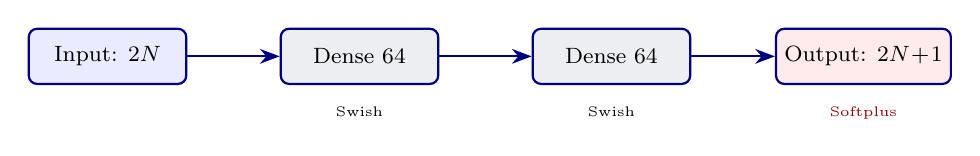
\begin{tikzpicture}[
    layer/.style={rectangle, draw=uzhblue, thick, fill=uzhgreylight,
        minimum width=2.0cm, minimum height=0.7cm, font=\footnotesize,
        rounded corners=3pt, inner sep=3pt},
    arr/.style={-{Stealth[length=2.5mm]}, thick, uzhblue}
]
    \node[layer, fill=blue!8] (in) at (0,0) {Input: $2N$};
    \node[layer] (h1) at (3.2,0) {Dense 64};
    \node[layer] (h2) at (6.4,0) {Dense 64};
    \node[layer, fill=red!8] (out) at (9.6,0) {Output: $2N\!+\!1$};

    \draw[arr] (in) -- (h1) node[midway, above, font=\tiny] {};
    \draw[arr] (h1) -- (h2) node[midway, above, font=\tiny] {};
    \draw[arr] (h2) -- (out) node[midway, above, font=\tiny] {};

    \node[below=0.15cm, font=\tiny] at (h1.south) {Swish};
    \node[below=0.15cm, font=\tiny] at (h2.south) {Swish};
    \node[below=0.15cm, font=\tiny, darkred] at (out.south) {Softplus};
\end{tikzpicture}
\end{center}

\vspace{0.5em}
\begin{itemize}
    \item \textbf{Hidden layers:} 2 layers $\times$ 64 units with \emphc{Swish} activation: $\text{swish}(x) = x \cdot \sigma(x)$
    \item \textbf{Output layer:} \emphc{Softplus} activation: $\ln(1 + e^x) > 0$
    \item Softplus ensures $k^{j\prime} > 0$, $\lambda > 0$, $\mu^j \geq 0$
    \item Total parameters: $(2N \cdot 64 + 64) + (64 \cdot 64 + 64) + (64 \cdot (2N+1) + 2N+1)$
\end{itemize}
\end{frame}

% --- Slide 23: Why Softplus? ---
\begin{frame}{Why Softplus for Output Activations?}
\begin{center}
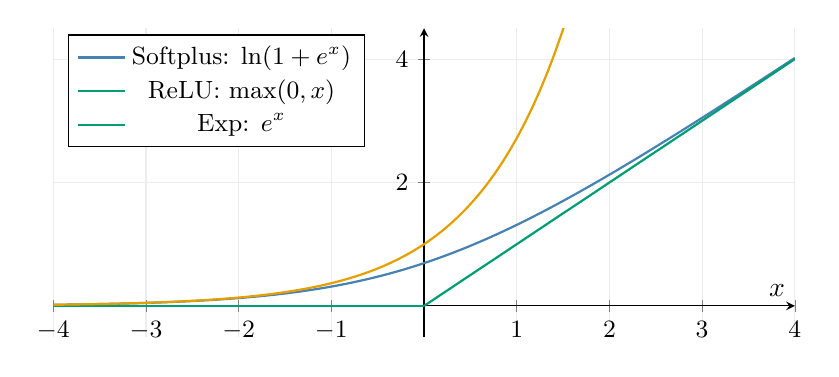
\begin{tikzpicture}
\begin{axis}[
    width=11cm, height=5.5cm,
    xlabel={$x$},
    xlabel style={font=\small},
    tick label style={font=\small},
    xmin=-4, xmax=4, ymin=-0.5, ymax=4.5,
    grid=major, grid style={gray!15},
    legend style={font=\small, at={(0.02,0.98)}, anchor=north west},
    axis lines=middle,
]
    \addplot[thick, softblue, domain=-4:4, samples=100]
        {ln(1+exp(x))};
    \addlegendentry{Softplus: $\ln(1+e^x)$}
    \addplot[thick, softgreen, domain=-4:0, samples=2]{0};
    \addplot[thick, softgreen, domain=0:4, samples=2]{x};
    \addlegendentry{ReLU: $\max(0,x)$}
    \addplot[thick, softorange, domain=-4:4, samples=100]
        {exp(x)};
    \addlegendentry{Exp: $e^x$}
\end{axis}
\end{tikzpicture}
\end{center}

\vspace{0.2em}
{\small
\textbf{Softplus} $\approx$ smooth ReLU: strictly positive, bounded gradients, no overflow risk (unlike $e^x$).
}
\end{frame}

% --- Slide 24: DEQN Loss for IRBC ---
\begin{frame}{DEQN Loss Function for the IRBC}
The loss is the \emphc{sum of squared residuals} across all equilibrium conditions:

\[
\boxed{
\ell_\rho = \frac{1}{B}\sum_{i=1}^{B} \left[\sum_{j=1}^{N} \bigl(\text{Euler}_j^{(i)}\bigr)^2 + \bigl(\text{ARC}^{(i)}\bigr)^2 + \sum_{j=1}^{N} \bigl(\text{FB}_j^{(i)}\bigr)^2\right]
}
\]

\vspace{0.3em}
where $B$ is the batch size and:
\begin{itemize}
    \item $\text{Euler}_j = \frac{\beta\,\E{\lambda' \text{MPK}' - (1-\delta)\mu'} + \mu}{\lambda(1+\Gamma_{k'})} - 1$
    \item $\text{ARC} = \sum_j [Y^j + (1-\delta)k^j - k^{j\prime} - \Gamma^j - c^j]$
    \item $\text{FB}_j = \mu^j + I^j - \sqrt{(\mu^j)^2 + (I^j)^2 + \varepsilon^2}$
\end{itemize}

\vspace{0.3em}
$\ell_\rho = 0$ iff all equilibrium conditions hold exactly.
\end{frame}

% --- Slide 25: Gauss-Hermite Quadrature ---
\begin{frame}{Gauss--Hermite Quadrature}
The Euler equation requires computing $\E{\cdot}$ over $N+1$ normal shocks.

\vspace{0.3em}
\textbf{Gauss--Hermite quadrature} in 1D:
\[
\E{f(\varepsilon)} = \int f(\varepsilon)\, \phi(\varepsilon)\,d\varepsilon \approx \sum_{q=1}^{Q} w_q \, f(\varepsilon_q)
\]

\vspace{0.3em}
\textbf{Tensor product} for $N+1$ dimensions:
\[
\E{f(\varepsilon^1, \ldots, \varepsilon^N, \varepsilon^{\text{agg}})} \approx \sum_{q_1=1}^{Q}\cdots\sum_{q_{N+1}=1}^{Q} \left(\prod_{d} w_{q_d}\right) f(\varepsilon_{q_1}, \ldots, \varepsilon_{q_{N+1}})
\]

\vspace{0.3em}
\begin{center}
\begin{tabular}{rrrr}
\toprule
$N$ & \textbf{Shocks} & $Q$ & \textbf{Quad.\ nodes} \\
\midrule
2 & 3 & 3 & 27 \\
4 & 5 & 3 & 243 \\
10 & 11 & 3 & $\sim 177$K \\
\bottomrule
\end{tabular}
\end{center}

{\small For large $N$: use monomial rules or QMC instead of tensor product.}
\end{frame}

% --- Slide 26: Computing Euler Expectation ---
\begin{frame}{Computing the Euler Expectation}
\textbf{Step-by-step} for each quadrature node $q$:

\vspace{0.3em}
\begin{enumerate}
    \item \textbf{Current state} $\bm{s}_t = (k^1, \ldots, k^N, z^1, \ldots, z^N)$
    \item \textbf{Current policy} $\mathcal{N}_\rho(\bm{s}_t) \to (k^{1\prime}, \ldots, k^{N\prime}, \lambda, \mu^1, \ldots, \mu^N)$
    \item \textbf{Next-period state} at node $q$:
    \[
    k^{j\prime}_q = k^{j\prime}, \qquad z^{j\prime}_q = \rho_z z^j + \sigma_e(\varepsilon^j_q + \varepsilon^{\text{agg}}_q)
    \]
    \item \textbf{Next-period policy:} evaluate $\mathcal{N}_\rho(\bm{s}_{t+1,q})$
    \item \textbf{Accumulate:} $\text{E-term} = \sum_q w_q \bigl[\lambda'_q \cdot \text{MPK}^j_q - (1-\delta)\mu^{j\prime}_q\bigr]$
\end{enumerate}

\vspace{0.3em}
{\small Each quadrature node requires a \emphc{forward pass} through the network---but all nodes in a batch can be evaluated in parallel.}
\end{frame}

% --- Slide 27: State Transition ---
\begin{frame}{State Transition}
\begin{center}
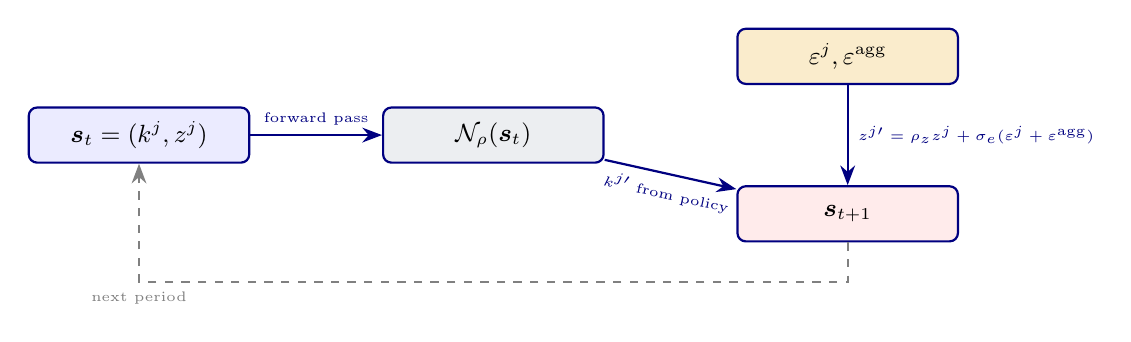
\begin{tikzpicture}[
    mlstep/.style={rectangle, draw=uzhblue, thick, fill=uzhgreylight,
        minimum width=2.8cm, minimum height=0.7cm, font=\small,
        rounded corners=3pt, inner sep=3pt},
    arr/.style={-{Stealth[length=2.5mm]}, thick, uzhblue}
]
    \node[mlstep, fill=blue!8] (st) at (0,0) {$\bm{s}_t = (k^j, z^j)$};
    \node[mlstep] (nn) at (4.5,0) {$\mathcal{N}_\rho(\bm{s}_t)$};
    \node[mlstep, fill=softorange!20] (shock) at (9,1) {$\varepsilon^j, \varepsilon^{\text{agg}}$};
    \node[mlstep, fill=red!8] (st1) at (9,-1) {$\bm{s}_{t+1}$};

    \draw[arr] (st) -- (nn) node[midway, above, font=\tiny] {forward pass};
    \draw[arr] (nn) -- (st1) node[midway, below, font=\tiny, sloped] {$k^{j\prime}$ from policy};
    \draw[arr] (shock) -- (st1) node[midway, right, font=\tiny] {$z^{j\prime} = \rho_z z^j + \sigma_e(\varepsilon^j + \varepsilon^{\text{agg}})$};

    \draw[arr, dashed, gray] (st1.south) -- ++(0,-0.5) -| (st.south)
        node[midway, below, font=\tiny, text=gray] {next period};
\end{tikzpicture}
\end{center}

\vspace{0.5em}
\begin{itemize}
    \item \textbf{Capital:} $k^{j\prime}$ is a policy output (endogenous)
    \item \textbf{TFP:} $z^{j\prime}$ evolves exogenously via AR(1) + shocks
    \item For simulation: draw $\varepsilon \sim \mathcal{N}(0,1)$
    \item For expectations: use quadrature nodes $\varepsilon_q$
\end{itemize}
\end{frame}

% --- Slide 28: Training Algorithm ---
\begin{frame}{Training Algorithm}
\begin{block}{Algorithm 1: DEQN Training for IRBC}
\begin{algorithmic}
\footnotesize
\STATE \textbf{Input:} Network $\mathcal{N}_\rho$, learning rate $\eta$, episodes $E$, GH nodes/weights
\STATE \textbf{Phase 1: Exogenous sampling}
\FOR{episode $e = 1, \ldots, E_1$}
    \STATE Draw $\bm{s}_i \sim \text{Uniform}(\mathcal{S})$ for $i = 1, \ldots, B$
    \STATE Compute loss $\ell_\rho = \frac{1}{B}\sum_i [\text{Euler}^2 + \text{ARC}^2 + \text{FB}^2]$
    \STATE Update: $\rho \leftarrow \rho - \eta\,\nabla_\rho \ell_\rho$ (Adam)
\ENDFOR
\STATE \textbf{Phase 2: Simulation-based sampling}
\FOR{episode $e = 1, \ldots, E_2$}
    \STATE Simulate: $\bm{s}_0 \to \bm{s}_1 \to \cdots \to \bm{s}_T$ using $\mathcal{N}_\rho$ and transition law
    \STATE Compute loss $\ell_\rho$ on simulated states
    \STATE Update: $\rho \leftarrow \rho - \eta\,\nabla_\rho \ell_\rho$ (Adam)
\ENDFOR
\STATE \textbf{Output:} Trained $\mathcal{N}_{\rho^\star}$
\end{algorithmic}
\end{block}
\end{frame}

% --- Slide 29: Scalability in N ---
\begin{frame}{Scalability in $N$}
\begin{center}
\begin{tabular}{rrrrl}
\toprule
$N$ & \textbf{States} & \textbf{Policies} & \textbf{NN params} & \textbf{Grid pts ($n\!=\!10$)} \\
\midrule
2 & 4 & 5 & $\sim$4.7K & $10^4$ \\
4 & 8 & 9 & $\sim$5.3K & $10^8$ \\
10 & 20 & 21 & $\sim$6.7K & $10^{20}$ \\
50 & 100 & 101 & $\sim$17K & $10^{100}$ \\
100 & 200 & 201 & $\sim$30K & $10^{200}$ \\
\bottomrule
\end{tabular}
\end{center}

\vspace{0.5em}
\begin{itemize}
    \item NN parameters grow \emphc{linearly} in $N$ (only input/output layers scale)
    \item Grid methods grow \emphc{exponentially}: $10^{2N}$ points
    \item DEQN training cost per step: $\mathcal{O}(|\rho| \cdot B \cdot Q^{N+1})$
    \item For large $N$: replace tensor-product GH with monomial rules or QMC
    \item Theoretical underpinning: \emphc{deep ReLU networks} beat the curse of dimensionality for sparse-grid-representable functions (Montanelli \& Du 2019)
\end{itemize}
\end{frame}

% --- Slide 30: From Brock-Mirman to IRBC ---
\begin{frame}{From Brock--Mirman to IRBC}
\begin{center}
\begin{tabular}{lll}
\toprule
& \textbf{Brock--Mirman} & \textbf{IRBC} \\
\midrule
Countries & 1 & $N$ \\
States & $(K, z)$ & $(k^1, \ldots, k^N, z^1, \ldots, z^N)$ \\
Policies & $C$ (or $s$) & $(k^{1\prime}, \ldots, k^{N\prime}, \lambda, \mu^1, \ldots, \mu^N)$ \\
Equations & 1 Euler & $N$ Euler $+$ 1 ARC $+$ $N$ FB \\
Constraints & none & irreversibility, adj.\ costs \\
Shocks & 1 & $N+1$ \\
Output act. & sigmoid & softplus \\
Analytical sol. & yes ($\delta=1$) & no \\
\bottomrule
\end{tabular}
\end{center}

\vspace{0.3em}
{\small The IRBC is a natural \emphc{scaling test} for the DEQN methodology.}
\end{frame}

% --- Slide 31: Recap ---
\begin{frame}{Recap: Three Building Blocks}
\begin{columns}[T]
\column{0.32\textwidth}
\begin{block}{Model}
\centering
\small
$N$-country IRBC with irreversible investment, adjustment costs, complete markets. $2N+1$ equilibrium equations.
\end{block}

\column{0.32\textwidth}
\begin{block}{Network}
\centering
\small
$\mathcal{N}_\rho: \R^{2N} \to \R^{2N+1}$ with swish hidden layers, softplus output. All policies in one forward pass.
\end{block}

\column{0.32\textwidth}
\begin{block}{Training}
\centering
\small
Two-phase: exogenous then simulation-based sampling. Adam optimizer on sum of squared residuals.
\end{block}
\end{columns}

\vspace{0.8em}
\begin{center}
$\Rightarrow$ \textbf{Next:} implementation in TensorFlow/Keras and results.
\end{center}
\end{frame}

% ============================================================================
% PART III: IMPLEMENTATION & RESULTS
% ============================================================================

% --- Slide 32: Section Divider ---
\begin{frame}{}
\vfill
\begin{center}
{\Huge \textcolor{uzhblue}{\textbf{Part III}}}\\[12pt]
{\LARGE Implementation \& Results}
\end{center}
\vfill
\end{frame}

% --- Slide 33: Notebook Overview ---
\begin{frame}{Notebook Overview}
\textbf{Two notebooks accompany this lecture:}

\vspace{0.5em}
\begin{enumerate}
    \item \texttt{01\_IRBC\_DEQN.ipynb} -- \emph{in-class walk-through}
    \begin{itemize}\itemsep1pt\vspace{2pt}
        \item Parameters \& steady state, Gauss--Hermite quadrature
        \item Keras network, production/consumption/adjustment-cost equations
        \item Cost function (Euler + ARC + FB), two-phase training loop
        \item Convergence, policy-function plots, economic diagnostics
    \end{itemize}

    \vspace{0.3em}
    \item \texttt{05\_IRBC\_Exercise.ipynb} -- \emph{hands-on exercise (blanks + solutions)}
    \begin{itemize}\itemsep1pt\vspace{2pt}
        \item Task 1: comparative statics on the deterministic steady state
        \item Task 2: inverse-loss weighting for multi-component losses (preview of ReLoBRaLo)
    \end{itemize}
\end{enumerate}

\vspace{0.4em}
{\small Self-contained: all equations implemented inline, no external imports.}
\end{frame}

% --- Slide 34: Parameters ---
\begin{frame}{Parameters}
\begin{center}
\begin{tabular}{llrl}
\toprule
\textbf{Symbol} & \textbf{Name} & \textbf{Value} & \textbf{Description} \\
\midrule
$\beta$ & Discount factor & 0.99 & Quarterly calibration \\
$\zeta$ & Capital share & 0.36 & Cobb--Douglas \\
$\delta$ & Depreciation & 0.01 & Low depreciation \\
$\rho_z$ & TFP persistence & 0.95 & Highly persistent \\
$\sigma_e$ & Shock std.\ dev. & 0.01 & Small shocks \\
$\kappa$ & Adjustment cost & 0.50 & Moderate costs \\
$\gamma_{\min}$ & Min IES & 0.25 & High risk aversion \\
$\gamma_{\max}$ & Max IES & 1.00 & Log utility \\
$k_{ss}$ & Steady-state capital & 1.00 & Normalization \\
\bottomrule
\end{tabular}
\end{center}

\vspace{0.3em}
{\small Pareto weights: $\tau^j = (A_{\text{tfp}} - \delta)^{1/\gamma_j} = c_{ss}^{1/\gamma_j}$.  At the symmetric steady state $c_{ss} = A_{\text{tfp}} - \delta$ for every country, so $\lambda_{ss} = \tau^j (c_{ss})^{-1/\gamma_j} = 1$ shared across all $j$ regardless of heterogeneous $\gamma_j$.}
\end{frame}

% --- Slide 35: Steady State ---
\begin{frame}{Steady State}
At steady state ($z^j = 0$, $k^j = k_{ss} = 1$, $\mu^j = 0$):

\vspace{0.3em}
\begin{align*}
A_{\text{tfp}} &= \frac{1 - \beta(1-\delta)}{\zeta\beta} = \frac{1 - 0.99 \cdot 0.99}{0.36 \cdot 0.99} \approx 0.0559 \\[4pt]
Y_{ss} &= A_{\text{tfp}} \cdot k_{ss}^\zeta = A_{\text{tfp}} \approx 0.0559 \\[4pt]
I_{ss} &= \delta \cdot k_{ss} = 0.01 \\[4pt]
c_{ss} &= Y_{ss} - I_{ss} \approx 0.0459
\end{align*}

\vspace{0.3em}
\textbf{Verification:} the ARC should be satisfied: $\sum_j [Y_{ss} - I_{ss} - c_{ss}] = 0$ \checkmark

\vspace{0.3em}
{\small The Euler equation at steady state gives the MPK $= 1/\beta$, which pins down $A_{\text{tfp}}$.}
\end{frame}

% --- Slide 36: Network Definition (Code) ---
\begin{frame}[fragile]{Network Definition (Keras)}
\begin{center}
\begin{minipage}{0.85\textwidth}
\begin{lstlisting}
N_COUNTRIES = 2
n_states = 2 * N_COUNTRIES      # = 4
n_policies = 2 * N_COUNTRIES + 1 # = 5

nn = keras.Sequential([
    keras.layers.Dense(64, activation='swish',
                       input_shape=(n_states,)),
    keras.layers.Dense(64, activation='swish'),
    keras.layers.Dense(n_policies,
                       activation='softplus')
])
\end{lstlisting}
\end{minipage}
\end{center}

\vspace{0.3em}
\begin{itemize}
    \item \texttt{swish}: $x \cdot \sigma(x)$ --- smooth, non-monotone, good gradients
    \item \texttt{softplus}: $\ln(1 + e^x)$ --- ensures all outputs $> 0$
    \item Output: $[k^{1\prime}, k^{2\prime}, \lambda, \mu^1, \mu^2]$
\end{itemize}
\end{frame}

% --- Slide 37: Production & Consumption (Code) ---
\begin{frame}[fragile]{Production \& Consumption}
\begin{columns}[T]
\column{0.48\textwidth}
\textbf{Production:}
\begin{lstlisting}[basicstyle=\footnotesize\ttfamily]
def production(k, z):
    return A_tfp * tf.exp(z) \
           * k**zeta
\end{lstlisting}

$Y^j = A_{\text{tfp}} \exp(z^j) (k^j)^\zeta$

\column{0.48\textwidth}
\textbf{Consumption (from FOC):}
\begin{lstlisting}[basicstyle=\footnotesize\ttfamily]
def consumption(lamb, j):
    tau = (A_tfp - delta)**(1./gammas[j])
    return (lamb/tau)**(-gammas[j])
\end{lstlisting}

$c^j = (\lambda / \tau^j)^{-\gamma_j}$
\end{columns}

\vspace{0.5em}
{\small All functions are vectorized over the batch dimension using TensorFlow operations.}
\end{frame}

% --- Slide 38: Adjustment Costs (Code) ---
\begin{frame}[fragile]{Adjustment Costs}
\begin{lstlisting}
def adj_cost(k, kp):
    j = kp / k - 1.0
    return 0.5 * kappa * j**2 * k

def adj_cost_kp(k, kp):
    return kappa * (kp / k - 1.0)

def adj_cost_k(k, kp):
    j = kp / k - 1.0
    return -0.5 * kappa * j * (j + 2.0)
\end{lstlisting}

\vspace{0.3em}
\textbf{Marginal product of capital:}
\begin{lstlisting}
def mpk(k, z, kp):
    Fk = zeta * A_tfp * tf.exp(z) \
         * k**(zeta - 1)
    return 1 - delta + Fk - adj_cost_k(k, kp)
\end{lstlisting}
\end{frame}

% --- Slide 39: Fischer-Burmeister (Code) ---
\begin{frame}[fragile]{Fischer--Burmeister Function}
\begin{lstlisting}
def fischer_burmeister(mu, I, eps=1e-4):
    return mu + I - tf.sqrt(mu**2 + I**2 + eps**2)
\end{lstlisting}

\vspace{0.3em}
\textbf{Investment:}
\begin{lstlisting}
def investment(k, kp):
    return kp - (1.0 - delta) * k
\end{lstlisting}

\vspace{0.3em}
The FB function is:
\begin{itemize}
    \item \emphc{Differentiable} everywhere for $\varepsilon>0$ (unlike $\min(\mu, I)$)
    \item \emphc{Exact zero set} at $\varepsilon=0$: $\mu \geq 0$, $I \geq 0$, $\mu \cdot I = 0$
    \item The small $\varepsilon$ prevents division-by-zero at the origin
\end{itemize}
\end{frame}

% --- Slide 40: Cost Function Structure ---
\begin{frame}[fragile]{Cost Function Structure}
\begin{lstlisting}[basicstyle=\footnotesize\ttfamily]
@tf.function
def compute_cost(states, nn):
    policies = nn(states)
    # Extract k', lambda, mu per country
    # For each GH quadrature node:
    #   Compute next state, evaluate nn,
    #   accumulate Euler integrand
    # Euler residual (relative error)
    # ARC: sum resources - uses = 0
    # FB: complementarity per country
    loss = mean(euler**2 + arc**2 + fb**2)
    return loss
\end{lstlisting}

\vspace{0.3em}
\textbf{Key point:} the entire computation graph is inside \texttt{@tf.function} for \emphc{automatic differentiation} via \texttt{GradientTape}.
\end{frame}

% --- Slide 41: Training: Exogenous Sampling ---
\begin{frame}{Training Phase 1: Exogenous Sampling}
\textbf{Phase 1} warms up the network on a broad state space.

\vspace{0.4em}
\begin{itemize}
    \item Draw $k^j \sim \text{Uniform}[k_{\min}, k_{\max}]$ and $z^j \sim \text{Uniform}[z_{\min}, z_{\max}]$
    \item Bounds chosen from steady-state analysis (e.g., $k \in [0.5, 1.5]$)
    \item The network learns a \emphc{rough approximation} of the policy
    \item Typical schedule: $10^4$--$5\!\cdot\!10^4$ iterations, learning rate $\eta \sim 10^{-3}$
\end{itemize}

\vspace{0.4em}
\textbf{Why start exogenous?}
\begin{itemize}
    \item At initialization, network weights are random $\Rightarrow$ policies are arbitrary
    \item Simulating with bad policies leads to \emphc{infeasible states} (negative capital, etc.)
    \item Exogenous sampling provides \emphc{stable training data} until the network is reasonable
\end{itemize}
\end{frame}

% --- Slide 42: Training: Simulation-Based ---
\begin{frame}{Training Phase 2: Simulation-Based Sampling}
\textbf{Phase 2} trains on the \emphc{ergodic distribution} of the model.

\vspace{0.4em}
\begin{itemize}
    \item Starting from Phase 1's endpoint, \emphc{simulate} the model forward
    \item Use simulated states as training data
    \item The network focuses on \emphc{economically relevant regions}
    \item Typical schedule: $5\!\cdot\!10^4$--$2\!\cdot\!10^5$ iterations with cosine annealing $\eta: 10^{-3} \!\to\! 10^{-5}$
    \item Switch trigger: $\max_j |\mathrm{Euler}^j| < 10^{-2}$ on a held-out sample
\end{itemize}

\vspace{0.4em}
\textbf{Advantages:}
\begin{itemize}
    \item Avoids wasting training effort in unreachable parts of the state space
    \item The training distribution \emphc{co-evolves} with the policy
\end{itemize}
\end{frame}

% --- Slide 43: Convergence: Loss Curves ---
\begin{frame}{Convergence: Four Training Strategies}
\begin{center}
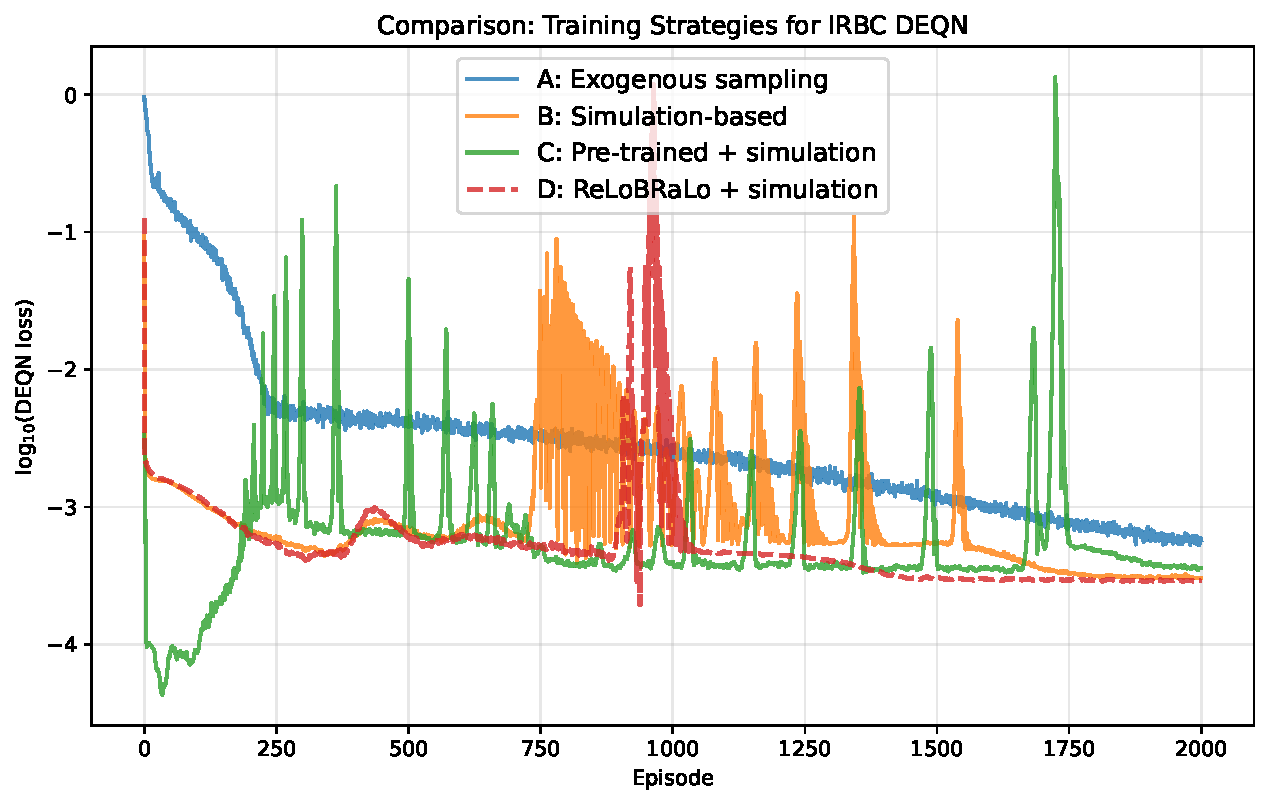
\includegraphics[width=0.95\linewidth]{../figures/irbc_4approach_loss.pdf}
\end{center}

\vspace{-0.4em}
{\footnotesize Generated by \texttt{01\_IRBC\_DEQN.ipynb} (cell 31).  Per-approach training-loss trajectories on the $N=2$ IRBC: \emphc{A} exogenous uniform sampling; \emphc{B} simulation-based sampling on the ergodic set; \emphc{C} pre-training on (A) followed by simulation-based refinement; \emphc{D} ReLoBRaLo on top of (C).  Each curve is the actual log10 of the multi-component DEQN loss, not a hand-drawn schematic.}
\end{frame}

% --- Slide 44: Convergence: Per-Equation ---
\begin{frame}{Convergence: Per-Equation Residuals}
\textbf{After training}, we evaluate residuals on a test set:

\vspace{0.5em}
\begin{center}
\begin{tabular}{lcc}
\toprule
\textbf{Residual} & \textbf{Mean $|\cdot|$} & \textbf{Max $|\cdot|$} \\
\midrule
Euler (country 1) & $\sim 10^{-4}$ & $\sim 10^{-3}$ \\
Euler (country 2) & $\sim 10^{-4}$ & $\sim 10^{-3}$ \\
ARC & $\sim 10^{-4}$ & $\sim 10^{-3}$ \\
FB (country 1) & $\sim 10^{-5}$ & $\sim 10^{-4}$ \\
FB (country 2) & $\sim 10^{-5}$ & $\sim 10^{-4}$ \\
\bottomrule
\end{tabular}
\end{center}

\vspace{0.3em}
\begin{itemize}
    \item Euler residuals $< 10^{-3}$ $\Rightarrow$ policy is accurate to within 0.1\%
    \item FB residuals near zero $\Rightarrow$ complementarity is well satisfied
    \item These are \emphc{relative errors}---interpretable as percentage deviations
\end{itemize}
\end{frame}

% --- Slide 45: Policy Functions ---
\begin{frame}{Policy Functions}
\textbf{After training,} we visualize the learned policies:

\vspace{0.3em}
\begin{columns}[T]
\column{0.48\textwidth}
\begin{itemize}
    \item \textbf{Capital policy} $k^{j\prime}$ vs.\ $k^j$:
    \begin{itemize}
        \item Near 45-degree line (close to replacement)
        \item Higher investment when TFP is high
    \end{itemize}
    \vspace{0.3em}
    \item \textbf{Shadow price} $\lambda$ vs.\ $z^j$:
    \begin{itemize}
        \item Decreasing in productivity (more output $\Rightarrow$ lower scarcity)
    \end{itemize}
\end{itemize}

\column{0.48\textwidth}
\begin{itemize}
    \item \textbf{Multiplier} $\mu^j$ vs.\ $k^j$:
    \begin{itemize}
        \item Near zero when $k$ is low (investment is positive)
        \item Positive when $k$ is high (irreversibility binds)
    \end{itemize}
    \vspace{0.3em}
    \item \textbf{Investment} $I^j$ vs.\ $k^j$:
    \begin{itemize}
        \item Positive most of the time
        \item Occasionally zero (constraint active)
    \end{itemize}
\end{itemize}
\end{columns}
\end{frame}

% --- Slide 46: Economic Diagnostics ---
\begin{frame}{Economic Diagnostics}
\begin{columns}[T]
\column{0.48\textwidth}
\textbf{Consumption sharing:}
\begin{itemize}
    \item Under complete markets, $c^1$ and $c^2$ should be \emphc{positively correlated}
    \item Perfect risk sharing: $c^1/c^2$ is constant
    \item With heterogeneous $\gamma$: ratio varies with $\lambda$
\end{itemize}

\vspace{0.5em}
\textbf{Trade balance:}
\begin{itemize}
    \item $\text{TB}^j = Y^j - c^j - I^j - \Gamma^j$
    \item Positive when country $j$ exports
    \item Sum across countries $= 0$
\end{itemize}

\column{0.48\textwidth}
\textbf{Ergodic distribution:}
\begin{itemize}
    \item Scatter plot of $(k^1, k^2)$ over long simulation
    \item Should concentrate near $(k_{ss}, k_{ss})$
    \item Correlation structure reveals risk-sharing patterns
\end{itemize}

\vspace{0.5em}
\textbf{Complementarity check:}
\begin{itemize}
    \item Plot $\mu^j$ vs.\ $I^j$
    \item Should lie on the axes: $\mu = 0$ or $I = 0$
    \item Fraction of time constraint binds
\end{itemize}
\end{columns}
\end{frame}

% --- Slide 47: Validation ---
\begin{frame}{Validation: Euler LHS vs.\ RHS}
\textbf{Key diagnostic:} compare both sides of the Euler equation on a test set.

\vspace{0.5em}
\begin{columns}[T]
\column{0.48\textwidth}
\textbf{LHS:} $\lambda \cdot (1 + \Gamma_{k'})$

\vspace{0.3em}
\textbf{RHS:} $\beta\,\E{\lambda' \cdot \text{MPK}' - (1-\delta)\mu'} + \mu$

\vspace{0.5em}
\textbf{Targets:}
\begin{itemize}
    \item Points should lie on the \emphc{45-degree line}
    \item Mean relative error $< 10^{-3}$
    \item Max relative error $< 10^{-2}$
\end{itemize}

\column{0.48\textwidth}
\textbf{Also check:}
\begin{itemize}
    \item ARC residual $\approx 0$ across all states
    \item $\mu^j \approx 0$ whenever $I^j > 0$ (complementarity)
    \item $I^j \geq 0$ everywhere (irreversibility)
\end{itemize}

\vspace{0.5em}
{\small These diagnostics confirm the network has learned a valid \emphc{approximate equilibrium}.}
\end{columns}
\end{frame}

\begin{frame}{Bridge to autodiff, sequence-space, and OLG lectures}
\textbf{What we leave with today.}  An IRBC DEQN that converges with NAS-tuned width and ReLoBRaLo-balanced loss components: the same recipe scales from $N=2$ to $N=10$ countries with no architectural change.

\vspace{0.4em}
\begin{columns}[T]
\column{0.48\textwidth}
\textbf{In the autodiff and OLG lectures.}
\begin{itemize}
    \item Reverse-mode automatic differentiation \emph{inside} the equilibrium loss (forward/reverse modes, JVP/VJP, AD pitfalls).
    \item \emph{Sequence-space} DEQNs: collapsing the recursion into a finite-horizon DAG (Brock--Mirman warm-up, then IRBC).
    \item OLG with DEQNs: the analytic 6-cohort benchmark of Krueger--K\"ubler (2004) and the 56-cohort benchmark of Azinovic, Gaegauf \& Scheidegger (2022).
\end{itemize}

\column{0.48\textwidth}
\textbf{Self-study extensions.}
\begin{itemize}
    \item Heterogeneous-agent solvers via Young's method (continuum approximated as a histogram).
    \item Continuum-of-agents DEQN.
    \item Krusell--Smith with deep learning.
\end{itemize}
\end{columns}
\end{frame}

% --- Slide 49: Questions ---
\begin{frame}{}
\begin{columns}[c]
\column{0.45\textwidth}
\begin{center}
{\Huge \textcolor{uzhblue}{\textbf{Questions?}}}

\vspace{1.0cm}
{\large Simon Scheidegger}\\[4pt]
{\small HEC, University of Lausanne}\\[4pt]
\url{https://sischei.github.io}

\vspace{0.6cm}
{\small Materials:~~\url{https://github.com/sischei/Deep_Learning_for_Solving_And_Estimating_Dynamic_Economic_Models}}
\end{center}

\column{0.45\textwidth}
\begin{center}
\textbf{Next up:}\\[6pt]
{\large AutoDiff $\to$ Sequence Space $\to$ OLG\\[2pt]
(Heterogeneous Agents = self-study)}\\[12pt]
\end{center}
\end{columns}
\end{frame}

\end{document}
